\documentclass[12pt]{article}
\usepackage{minted}
\usepackage{graphicx}
\usepackage{mathtools}
\usepackage{amsfonts}

\begin{document}
    \title{CS 559 Homework 1}
    \author{Stephen Szemis}
    \date{October 1, 2020}
    \maketitle

    \paragraph{Problem 1:} ~\\
    Suppose you have a set of medical data and you are looking at the relation 
    between being a football player and having a concussion at some point in life. 
    Say event A is that you have had a concussion at some point and event B is that 
    you are a football player. \(P(A | B)\) is therefore the probability that you’ve 
    had a concussion given that you are a football player; while \(P(B | A)\) is the 
    probability that you are a football player given that you’ve had a concussion. 
    We know that football players are more likely to have concussions when compared 
    to the general population, so it’s pretty clear that \(P(A | B)\) is not the same 
    as \(P(B | A)\).

    \paragraph{Problem 2:} ~\\
    Show relation between independence and correlation.
    \begin{enumerate}
        \item 
        Given X and Y are two continuous independent random variables we know
        \[ f(X, Y) = f_x(X)f_y(Y) \]
        \[ Cov(X, Y) = E(XY)-E(X)E(Y) \]
        \(E(XY)=E(X)E(Y) - E(X)E(Y)\) for independent variables therefore
        \(Cov(X,Y) = E(X)(Y) - E(X)E(Y) = 0\) which show that they are uncorrelated.
        \item
        Suppose \(X \sim Uniform[-1, 1]\) and \(Y = X^2\)

        First let's show that this is uncorrelated.
        \[ Cov(X,Y) = E(XY) - E(X)E(Y) \]
        \[ Cov(X,Y) = E(X*X^2) - E(X)E(X^2) = E(X^3)  - E(X)E(X^2) \]
        \[ E(X) = \frac{1}{2}(1 - 1) = 0 \]
        \[ E(X^3) = \frac{1 - 1}{(3+1)(-2)} = 0 \]
        \[ Cov(X,Y) = 0 - 0*E(X^2) = 0 \]
        So they are uncorrelated, and they are clearly not independent
        since X determines Y.
    \end{enumerate}

    \paragraph{Problem 3:} ~\\
    We start from the simple Discriminant function
    \[ g_j(\mathbf{x}) = ln(P( \mathbf{x} | \omega _{j})) + ln(\omega _{j}) \]
    We need to expand this out. If we want the probability of a series of independent events, 
    we can simply multiply the probability of each "individual" event. So we get.\dots
    \[ 
        P( \mathbf{x} | \omega _{j}) = \prod_{i=1}^{d} P( x_{i} | \omega _{j})
    \]
    Now we need to know what \( P( x_{i} | \omega _{j}) \) is in terms of \( P_{ij} \) (as defined 
    in the problem). \( P_{ij} \) is the probability of \( x_i = 1 \) given event \( \omega_j \).
    In order to find the probability of any value of \( x_i \) we need to account for both when it 
    could be 0 or 1. This is very similar to the binomial distribution but for a very special case.
    We can formalize this logic as:
    \[
        P( x_{i} | \omega _{j}) = \binom{1}{1} (P_{ij})^{x_{i}} * (1 - P_{ij})^{1 - x_{i}}
    \]
    Simplified and plugged into the previous product we get.
    \[
        P( \mathbf{x} | \omega _{j}) = \prod_{i=1}^{d} (P_{ij})^{x_{i}} * (1 - P_{ij})^{1 - x_{i}}
    \]
    Which, when placed in our Discriminant function gives us.
    \[
        g_j(\mathbf{x}) = ln(\prod_{i=1}^{d} (P_{ij})^{x_{i}} * (1 - P_{ij})^{1 - x_{i}}) + ln(\omega _{j})
    \]
    Thanks to logarithmic properties we can simplify this into.
    \[
        g_j(\mathbf{x}) = \sum_{i=1}^{d} \big( x_{i}ln(P_{ij}) + (1 - x_{i})ln(1 - P_{ij}) \big) + ln(P(\omega _{j}))
    \]
    Which with one more division and some splitting can become our final equation.
    \[
        g_j(\mathbf{x}) = \sum_{i=1}^{d} \frac{(1 - x_{i})}{(1 - x_{i})} * \big( x_{i}ln(P_{ij}) + (1 - x_{i})ln(1 - P_{ij}) \big) + ln(P(\omega _{j}))
    \]
    \[
        g_j(\mathbf{x}) = \sum_{i=1}^{d} \big( x_{i} \frac{ln(P_{ij})}{(1 - x_{i})} \big) +  \sum_{i=1}^{d} ln(1 - P_{ij})+ ln(P(\omega _{j}))
    \]

    \paragraph{Problem 4: } ~\\
    We will first list all known information.
    \[ P(x|\omega_{1}) = N(4, 1) \]
    \[ P(x|\omega_{2}) = N(8, 1) \]
    \[ P(\omega_{2}) = \frac{1}{4} \]
    \[
        \lambda = \begin{bmatrix}
            0 & 1 \\
            3 & 0
        \end{bmatrix}
    \]
    We can find the prior for \(\omega_1\) easily from the other prior.
    \[ P(\omega_{1}) = \frac{3}{4} \]
    
    We can write the Normal distribution explicitly.
    \[
        P(x|\omega_{1}) = \frac{1}{2\pi}e^{-\frac{(x-4)^{2}}{2}}
    \]
    \[
        P(x|\omega_{1}) = \frac{1}{2\pi}e^{-\frac{(x-10)^{2}}{2}}
    \]
    And we can then calculate the LHS of our decision rule.
    \[
        \frac{P(x|\omega_{1})}{P(x|\omega_{2})} 
        = \frac
        { \frac{1}{2\pi}e^{-\frac{(x-4)^{2}}{2}} }
        { \frac{1}{2\pi}e^{-\frac{(x-10)^{2}}{2}} }
        = \frac
        {e^{-\frac{(x-4)^{2}}{2}}}
        {e^{-\frac{(x-10)^{2}}{2}}}
        = e^{-\frac{(x-4)^{2}}{2} + \frac{(x-10)^{2}}{2} }
    \]
    \[
        \frac{P(x|\omega_{1})}{P(x|\omega_{2})}
        = e^{ \frac{(x-10)^{2} - (x-4)^{2}}{2} }
        = e^{ \frac{x^2 - 20x + 100 - x^2 + 8x - 16}{2} }
        = e^{-6x + 42}
    \]
    Doing the same for RHS of our decision rule, we get.
    \[
        \frac{ \lambda_{12} - \lambda_{22} }{ \lambda_{21} - \lambda_{11}}
        \frac{P(\omega_{2})}{P(\omega_{1})}
        = \frac{1 - 0}{3 - 0}\frac{1}{3} = \frac{1}{9}
    \]
    So we have the full inequality.
    \[
        e^{-6x + 42} > \frac{1}{9}
    \]
    We can take the natural log of both sides, since it is an 
    monotonically increasing function.
    \[
        -6x + 42 > ln(\frac{1}{9})
    \]
    \[
        -6x + 42 > -2.197
    \]
    \[
        x < 7.366
    \]

    \paragraph{Problem 5:}
    \begin{enumerate}
        \item
        The normal decision rule is the following
        \[
            \text{Choose } \omega_i \text{ if }
            P(\omega_i | x) \ge P(\omega_j | x), \forall j
        \]
        This is known. However, we need to add an addition rule
        deciding whether rejection is more optimal when compared to 
        a normal classification. In essence, we need to compare the Risk
        of rejection versus the Risk of classification. The two cases 
        condition risk is as follows.
        \[
            R(\alpha_{c+1} | x) = \sum_{j=1}^{c} \lambda_r P(\omega_j | x) = \lambda_r
        \]
        \[
            R(\alpha_{i} | x) = \sum_{i \neq j} \lambda_s P(\omega_j | x) = \lambda_s (1 - P(\omega_j | x))
        \]
        We create our inequality.
        \[
            R(\alpha_{c+1} | x) \ge R(\alpha_{i} | x)
        \]
        And solve.
        \[ \lambda_r \ge \lambda_s (1 - P(\omega_j | x)) \]
        \[ \frac{\lambda_r}{\lambda_s} \ge 1 - P(\omega_j | x) \]
        \[ P(\omega_j | x) \ge 1 - \frac{\lambda_r}{\lambda_s} \]
        So our decision rule can be written as
        \[ \text{Choose } \omega_i \text{ if }
            P(\omega_i | x) \ge P(\omega_j | x), \forall j \]
        \[ \text{and } P(\omega_j | x) \ge 1 - \frac{\lambda_r}{\lambda_s} \]
        \item
        If \( \lambda_r = 0 \) then our second condition can never be met, since the RHS of our
        inequality is 1, and the LHS is a probability (i.e. less then 1).
        This means that we will always choose to reject, since there is no cost to 
        rejecting.
        \item
        If \( \lambda_r > \lambda_s \) then the ratio is greater then 1, meaning the RHS
        of our inequality is less then 0. Which means the cost of rejection is so high as to never
        be worth it. It is always more optimal to classify something in that case.
    \end{enumerate}

    \paragraph{Problem 6:}~\\
    Maximum Likelihood Estimation
    \begin{enumerate}
        \newcommand{\temp}{\int h(x) \, \mathrm{exp}\left\{ \eta^{T} T(x) \right\} \mathrm{d}x}
        \item
        \[ p(x, \eta) = h(x) \, \mathrm{exp}\left\{ \eta^{T} T(x) - A(\eta) \right\} \]
        Because \(p(x, \eta)\) is a probability density function, we know that the integral of it is 
        always equal to 1 (thank you for this hint professor!). So, using that we have.
        \[ \int h(x) \, \mathrm{exp}\left\{ \eta^{T} T(x) - A(\eta) \right\} \mathrm{d}x = 1 \]
        \[ \mathrm{exp}\left\{ - A(\eta)  \right\} \int h(x) \, \mathrm{exp}\left\{ \eta^{T} T(x) \right\} \mathrm{d}x = 1 \]
        \[ \mathrm{exp}\left\{ A(\eta)  \right\} = \int h(x) \, \mathrm{exp}\left\{ \eta^{T} T(x) \right\} \mathrm{d}x \]
        \[ A(\eta) = \mathrm{ln} \int h(x) \, \mathrm{exp}\left\{ \eta^{T} T(x) \right\} \mathrm{d}x \]
        \item
        \[ \frac{\partial}{\partial\,\eta} A(\eta) = \frac{1}{\temp}*\,\frac{\partial}{\partial\,\eta} \temp \]
        \[ = \frac{1}{\temp} * \int h(x) T(x) \, \mathrm{exp}\left\{ \eta^{T} T(x) \right\} \mathrm{d}x \]
        \[ = \frac{1}{\mathrm{exp} \left\{ A(\eta) \right\} } * \int h(x) T(x) \, \mathrm{exp}\left\{ \eta^{T} T(x) \right\} \mathrm{d}x \]
        \[ = \int h(x) T(x) \, \mathrm{exp}\left\{ \eta^{T} T(x) - A(x) \right\} \]
        \[ = \int p(x, \eta) T(x) \mathrm{d}x \]
        \[ = E[T(x)] \]
        \item
        \[ l(\eta) = \sum_{k=1}^{n} ln(p(x_k | \eta)) \]
        \[ = \sum_{k=1}^{n} ln(h(x_k)) + \eta T(x_k) - A(\eta) \]
        \[ = \sum_{k=1}^{n} ln(h(x_k)) + \eta \sum_{k=1}^{n} T(x_k) - (n * A(\eta)) \]
        Take derivative
        \[ = 0 + \sum_{k=1}^{n}T(x_k) - n * E[T(x)] = 0\]
        \[ A'(\eta) = E[T(x)] = \frac{1}{n}\sum_{k=1}^{n}T(x_k) \]
    \end{enumerate}
    \paragraph{Problem 7:}~\\
    Logistic Regression
    \begin{enumerate}
        \item It's a derivative of the log likelihood function.
        \item 
        First the code
        \inputminted{python}{hw1.py}

        And here are the graphs, note that the dashed line marks where our
        decision boundary is.
        \begin{center}
        

            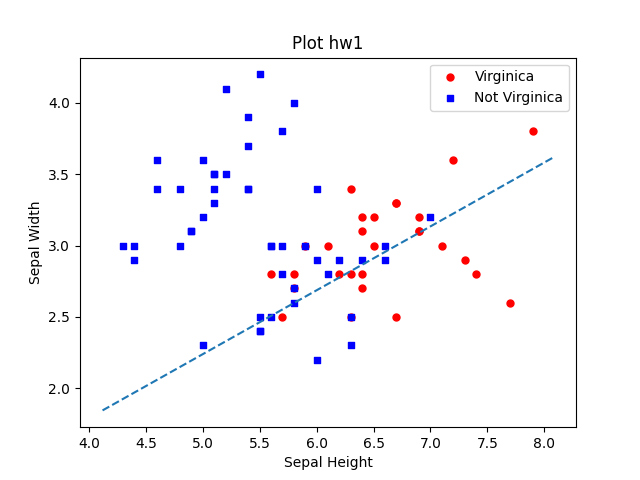
\includegraphics[width=10cm]{Figure_1.png}
        
        
            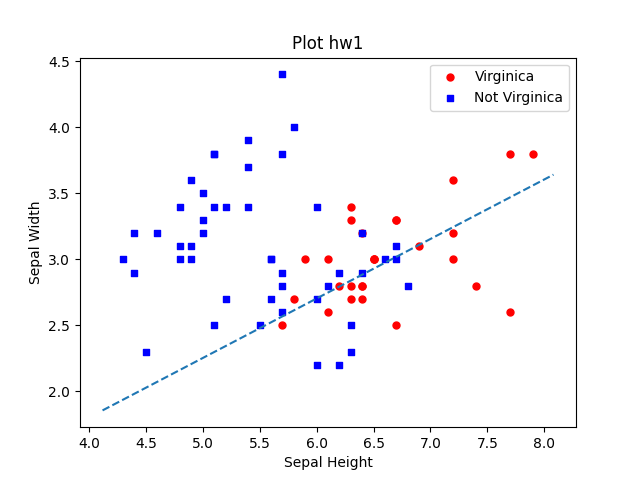
\includegraphics[width=10cm]{Figure_2.png}
        \end{center}
        From my testing we find an accuracy around 68\%.
    \end{enumerate}

\end{document}